% !TeX root = ./main.tex
% !TeX spellcheck = de_DE

\documentclass[fontzize=12pt,paper=a4,twoside=false]{article}
\usepackage{ngerman}
\usepackage{graphicx}
\graphicspath{{assets/}}
\usepackage{fullpage}
\usepackage{hyperref}
\hypersetup{
    colorlinks=true,
    linkcolor=blue,
    filecolor=magenta,      
    urlcolor=cyan,
}

\title{Amateurfunklehrgang}
\author{Konrad Gralher}

\begin{document}
\begin{titlepage}
    \bfseries\Huge\centering{
    Amateurfunklehrgang 2021\\
    \vskip3cm
    \huge\itshape{
        Konrad Gralher\\
        }
    }    

    \begin{figure}
        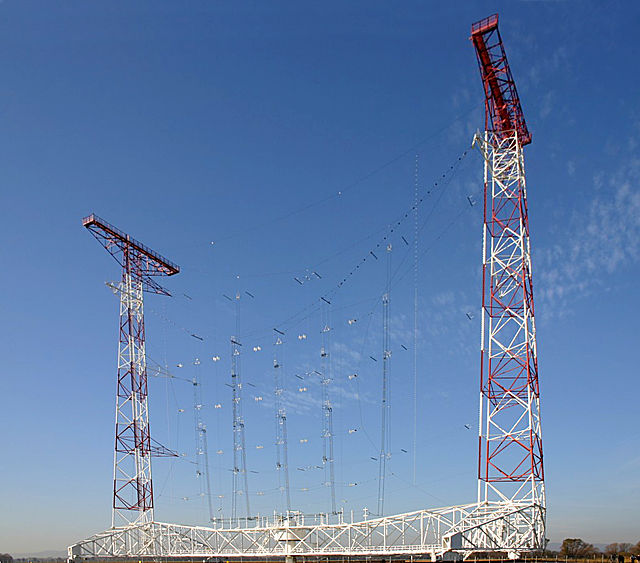
\includegraphics[]{assets/640px-Moosbrunn_SW_Antenna}
        \caption{Kurzwellenstation Moosbrunn}  
    \end{figure}        
\end{titlepage}
% !TeX root = ../main.tex
% !TeX spellcheck = de_DE

{\bfseries\Huge\centering{
Kurzwellenausbreitung\\ 
\vskip 1cm
\huge\itshape{
    Klasse E und A\\
    }
}}
\begin{figure}
    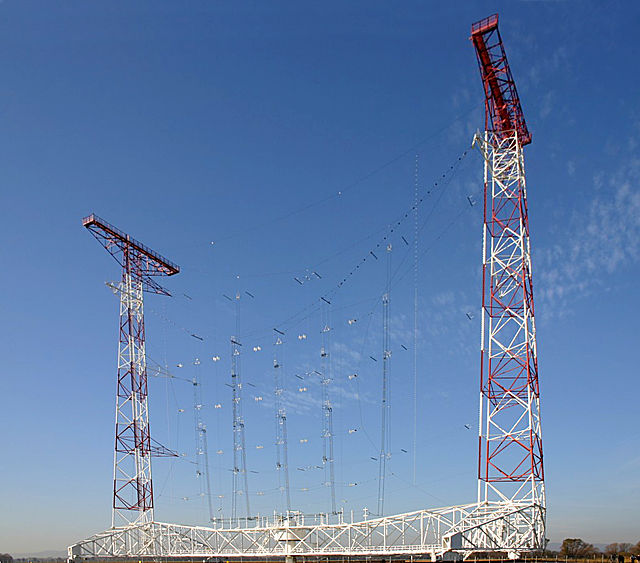
\includegraphics[]{assets/640px-Moosbrunn_SW_Antenna}
    \caption{Kurzwellenstation Moosbrunn}  
\end{figure}        
\newpage
\part[]{Wellenausbreitung}

    Die Sendungen im Kurzwellenbereich werden in der Ionosphäre reflektiert. 
    Ukw besitzt diese Eigenschaften nicht, da die Wellen sich eher wie Licht ausbreiten(bedingt durch kleinere Wellenlänge). Durch Reflektionen der Kurzwelle an der Ionosphäre
    sind deutlich größere Reichweiten möglich(DX Betrieb).
    \vspace{0.1cm}
    \subsection[]{Wellenarten}
        Bei der Kurzwellenausbreitung spielen zwei Arten der Welle eine Rolle.
        \begin{enumerate}
            \item Raumwelle
            \begin{itemize}
                \item bezeichnet alle sich im Raum ausbreitende Wellen(große Reichweite wenn in Skip Distanz)
                \item hat Relevanz für KW(Kurzwelle)
                \item die Ausbreitung hängt von dem Einfallswinkel der Strahlen ab
                \begin{itemize}
                    \item Die kritische Frequenz kann durch folgende Formel berechnet werden:\newline \( MUF \approx \frac{f k}{sin \alpha }\)	\newline {\it MUF = maximal usable frequencie} 
                \end{itemize}
            \end{itemize}
            \item Bodenwelle
            \begin{itemize}
                \item bezeichnet die sich am Boden mit der Erdkrümmung ausbreitende Welle (kleine Reichweite)
                \item werden mit zunehmender Frequenz gedämpft
                \item wird im Lang- und Mittelwellebereich aufgenutzt
                \item geht über den Geografischen Horizont hinaus
            \end{itemize}
        \end{enumerate}
    \subsection[]{Ionosphäre}
        Die für die Kurzwellenausbreitung Relevanten Schichten, befinden sich etwa in 100-500km Höhe.
        Dort findet eine Brechung und anschließend eine Reflektion statt.
        Die Bedingungen auf den jeweiligen Bänder hängt von der Jahreszeit der Frequenz, Sonnenflecken und Tageszeit ab. \newline
        \href{https://www.darc.de/fileadmin/filemounts/referate/ajw/Onlinelehrgang/e09/Bild9-2.gif}{Verschiedene Schichte der Ionosphäre.}

            \subsubsection[]{D-Schicht}
            {\it D = dämpfend oder doof\newline aber auch schnell weg } \newline
            Die D-Schicht sorgt Tagsüber für Dämpfungen auf der unteren Kurzwelle. Mit Sonnenuntergang verschwindet diese sehr schnell. Kann bei sehr starker Ausbreitung auch die gesamte Kurzwelle betreffen. 
            (Mögel-Dellinger-Effekt) Mit einer Leistungserhöhung kann man diesen Effekt ausgleichen.
            Fading beschreibt das Überlagern der Raum und Bodenwelle was das Signal in seiner Amplitude schwanken lässt.
            \begin{enumerate}
                \item 160 - 80m starke Dämpfung brauchen dafür aber schwache F2 Schicht (Nachtband)
                \item 40m mäßige Dämpfung (Übergangsband)
                \item 20 - 10m wenig gedämpft brauchen aber eine starke F2 Schicht (Tagesbänder)
            \end{enumerate}
            \subsubsection[]{F- und E-Schicht}
            Die F Schicht hat den größten Anteil an Reflektionen. \newline
            Die F2 Schicht sorgt für interkontinentale Funkverbindungen.(größte Höhenausdehnung)(400km Höhe) Außerdem ist sie weniger anfällig für Sonnenflecken, da sie träger als andere Schichten ist. (Skip Distanz: 4000km)
            \newline 
            Die F-Schicht dezimiert sich während der Nacht. Deshalb ist sie kurz vor Sonnenaufgang am geringsten. In den Tagesstunden kann sie sich aber bei intensiver Sonneneinstrahlung aufspalten und bildet so die F1 und F2 Schicht.
            Dabei ist zu beachten, dass die tiefer liegende F1 Schicht die von der F2 Schicht reflektierten Strahlen dämpft. Es entstehen sogenannte \dq short skips\dq.

    \subsubsection[]{Tote Zone}
        Die Tote Zone bezeichnet die Zone zwischen den Skips die weder von der Bodenwelle weder noch von der Raumwelle erreicht werden kann.
    \subsubsection[]{Fading}
    \subsubsection[]{Sonnenflecken}
        Je mehr Flecken
        \begin{list}{}{}
            \item umso mehr UV-Strahlen 
            \item umso stärkere F2-Schicht
            \item umso besser funken ...
        \end{list}
        Ein Zylkus der Sonnenflecken dauert im Durschnitt 11 Jahre.
    \subsubsection[]{Solarer Flux}
    \subsection[]{Einzelne Bänder}

    \subsection[]{Übersicht}
    \begin{enumerate}
        \item F2 400km
        \item F1 200km
        \item E (sparodic E) 100km
        \item D 70-80km
    \end{enumerate}
    Alle Schichten sind abhängig von der Sonne. Durch unterschiedlich schnellen Abbau der Schichten verändern sich die Bedinungen im Verlauf des Tages.
\end{document}